% Options for packages loaded elsewhere
\PassOptionsToPackage{unicode}{hyperref}
\PassOptionsToPackage{hyphens}{url}
%
\documentclass[
  11pt,
  ignorenonframetext,
]{beamer}
\usepackage{pgfpages}
\setbeamertemplate{caption}[numbered]
\setbeamertemplate{caption label separator}{: }
\setbeamercolor{caption name}{fg=normal text.fg}
\beamertemplatenavigationsymbolsempty
% Prevent slide breaks in the middle of a paragraph
\widowpenalties 1 10000
\raggedbottom
\setbeamertemplate{part page}{
  \centering
  \begin{beamercolorbox}[sep=16pt,center]{part title}
    \usebeamerfont{part title}\insertpart\par
  \end{beamercolorbox}
}
\setbeamertemplate{section page}{
  \centering
  \begin{beamercolorbox}[sep=12pt,center]{part title}
    \usebeamerfont{section title}\insertsection\par
  \end{beamercolorbox}
}
\setbeamertemplate{subsection page}{
  \centering
  \begin{beamercolorbox}[sep=8pt,center]{part title}
    \usebeamerfont{subsection title}\insertsubsection\par
  \end{beamercolorbox}
}
\AtBeginPart{
  \frame{\partpage}
}
\AtBeginSection{
  \ifbibliography
  \else
    \frame{\sectionpage}
  \fi
}
\AtBeginSubsection{
  \frame{\subsectionpage}
}
\usepackage{amsmath,amssymb}
\usepackage{iftex}
\ifPDFTeX
  \usepackage[T1]{fontenc}
  \usepackage[utf8]{inputenc}
  \usepackage{textcomp} % provide euro and other symbols
\else % if luatex or xetex
  \usepackage{unicode-math} % this also loads fontspec
  \defaultfontfeatures{Scale=MatchLowercase}
  \defaultfontfeatures[\rmfamily]{Ligatures=TeX,Scale=1}
\fi
\usepackage{lmodern}
\usetheme[]{metropolis}
\ifPDFTeX\else
  % xetex/luatex font selection
\fi
% Use upquote if available, for straight quotes in verbatim environments
\IfFileExists{upquote.sty}{\usepackage{upquote}}{}
\IfFileExists{microtype.sty}{% use microtype if available
  \usepackage[]{microtype}
  \UseMicrotypeSet[protrusion]{basicmath} % disable protrusion for tt fonts
}{}
\makeatletter
\@ifundefined{KOMAClassName}{% if non-KOMA class
  \IfFileExists{parskip.sty}{%
    \usepackage{parskip}
  }{% else
    \setlength{\parindent}{0pt}
    \setlength{\parskip}{6pt plus 2pt minus 1pt}}
}{% if KOMA class
  \KOMAoptions{parskip=half}}
\makeatother
\usepackage{xcolor}
\newif\ifbibliography
\usepackage{color}
\usepackage{fancyvrb}
\newcommand{\VerbBar}{|}
\newcommand{\VERB}{\Verb[commandchars=\\\{\}]}
\DefineVerbatimEnvironment{Highlighting}{Verbatim}{commandchars=\\\{\}}
% Add ',fontsize=\small' for more characters per line
\newenvironment{Shaded}{}{}
\newcommand{\AlertTok}[1]{\textcolor[rgb]{1.00,0.00,0.00}{\textbf{#1}}}
\newcommand{\AnnotationTok}[1]{\textcolor[rgb]{0.38,0.63,0.69}{\textbf{\textit{#1}}}}
\newcommand{\AttributeTok}[1]{\textcolor[rgb]{0.49,0.56,0.16}{#1}}
\newcommand{\BaseNTok}[1]{\textcolor[rgb]{0.25,0.63,0.44}{#1}}
\newcommand{\BuiltInTok}[1]{\textcolor[rgb]{0.00,0.50,0.00}{#1}}
\newcommand{\CharTok}[1]{\textcolor[rgb]{0.25,0.44,0.63}{#1}}
\newcommand{\CommentTok}[1]{\textcolor[rgb]{0.38,0.63,0.69}{\textit{#1}}}
\newcommand{\CommentVarTok}[1]{\textcolor[rgb]{0.38,0.63,0.69}{\textbf{\textit{#1}}}}
\newcommand{\ConstantTok}[1]{\textcolor[rgb]{0.53,0.00,0.00}{#1}}
\newcommand{\ControlFlowTok}[1]{\textcolor[rgb]{0.00,0.44,0.13}{\textbf{#1}}}
\newcommand{\DataTypeTok}[1]{\textcolor[rgb]{0.56,0.13,0.00}{#1}}
\newcommand{\DecValTok}[1]{\textcolor[rgb]{0.25,0.63,0.44}{#1}}
\newcommand{\DocumentationTok}[1]{\textcolor[rgb]{0.73,0.13,0.13}{\textit{#1}}}
\newcommand{\ErrorTok}[1]{\textcolor[rgb]{1.00,0.00,0.00}{\textbf{#1}}}
\newcommand{\ExtensionTok}[1]{#1}
\newcommand{\FloatTok}[1]{\textcolor[rgb]{0.25,0.63,0.44}{#1}}
\newcommand{\FunctionTok}[1]{\textcolor[rgb]{0.02,0.16,0.49}{#1}}
\newcommand{\ImportTok}[1]{\textcolor[rgb]{0.00,0.50,0.00}{\textbf{#1}}}
\newcommand{\InformationTok}[1]{\textcolor[rgb]{0.38,0.63,0.69}{\textbf{\textit{#1}}}}
\newcommand{\KeywordTok}[1]{\textcolor[rgb]{0.00,0.44,0.13}{\textbf{#1}}}
\newcommand{\NormalTok}[1]{#1}
\newcommand{\OperatorTok}[1]{\textcolor[rgb]{0.40,0.40,0.40}{#1}}
\newcommand{\OtherTok}[1]{\textcolor[rgb]{0.00,0.44,0.13}{#1}}
\newcommand{\PreprocessorTok}[1]{\textcolor[rgb]{0.74,0.48,0.00}{#1}}
\newcommand{\RegionMarkerTok}[1]{#1}
\newcommand{\SpecialCharTok}[1]{\textcolor[rgb]{0.25,0.44,0.63}{#1}}
\newcommand{\SpecialStringTok}[1]{\textcolor[rgb]{0.73,0.40,0.53}{#1}}
\newcommand{\StringTok}[1]{\textcolor[rgb]{0.25,0.44,0.63}{#1}}
\newcommand{\VariableTok}[1]{\textcolor[rgb]{0.10,0.09,0.49}{#1}}
\newcommand{\VerbatimStringTok}[1]{\textcolor[rgb]{0.25,0.44,0.63}{#1}}
\newcommand{\WarningTok}[1]{\textcolor[rgb]{0.38,0.63,0.69}{\textbf{\textit{#1}}}}
\usepackage{graphicx}
\makeatletter
\def\maxwidth{\ifdim\Gin@nat@width>\linewidth\linewidth\else\Gin@nat@width\fi}
\def\maxheight{\ifdim\Gin@nat@height>\textheight\textheight\else\Gin@nat@height\fi}
\makeatother
% Scale images if necessary, so that they will not overflow the page
% margins by default, and it is still possible to overwrite the defaults
% using explicit options in \includegraphics[width, height, ...]{}
\setkeys{Gin}{width=\maxwidth,height=\maxheight,keepaspectratio}
% Set default figure placement to htbp
\makeatletter
\def\fps@figure{htbp}
\makeatother
\setlength{\emergencystretch}{3em} % prevent overfull lines
\providecommand{\tightlist}{%
  \setlength{\itemsep}{0pt}\setlength{\parskip}{0pt}}
\setcounter{secnumdepth}{-\maxdimen} % remove section numbering
\ifLuaTeX
  \usepackage{selnolig}  % disable illegal ligatures
\fi
\IfFileExists{bookmark.sty}{\usepackage{bookmark}}{\usepackage{hyperref}}
\IfFileExists{xurl.sty}{\usepackage{xurl}}{} % add URL line breaks if available
\urlstyle{same}
\hypersetup{
  pdftitle={Metapoblaciones},
  pdfauthor={Gerardo Martín},
  hidelinks,
  pdfcreator={LaTeX via pandoc}}

\title{Metapoblaciones}
\subtitle{Modelos}
\author{Gerardo Martín}
\date{28-07-2023}

\begin{document}
\frame{\titlepage}

\hypertarget{intro}{%
\subsection{Intro}\label{intro}}

\begin{frame}{Intro}
\begin{itemize}
\item
  Modelos representan fracción de parches ocupados en un sistema de
  parches de hábitat
\item
  Los modelos son mecanínsticos

  \begin{itemize}
  \tightlist
  \item
    Representan explícitamente parte del fenómeno
  \end{itemize}
\item
  Basados en ecuaciones diferenciales

  \begin{itemize}
  \tightlist
  \item
    Tiempo contínuo vs Tiempo discreto
  \end{itemize}
\end{itemize}
\end{frame}

\hypertarget{recordatorio}{%
\subsection{Recordatorio}\label{recordatorio}}

\begin{frame}{Recordatorio}
Ecuación diferencial:

\[\frac{dN}{dt} = r N\]

\begin{itemize}
\item
  \(dN/dt = N'(t)\), es la derivada de \(N\) con respecto de \(t\)

  \begin{itemize}
  \tightlist
  \item
    Es el cambio neto de la población por unidad de tiempo
  \end{itemize}
\item
  \(r\) es la tasa instantánea de cambio de \(N\)

  \begin{itemize}
  \tightlist
  \item
    Número nuevo de individos per cápita que ingresarán a población
  \end{itemize}
\end{itemize}
\end{frame}

\hypertarget{ejemplo-con-funciuxf3n-lineal}{%
\subsection{Ejemplo con función
lineal}\label{ejemplo-con-funciuxf3n-lineal}}

\begin{frame}{Ejemplo con función lineal}
\[f(x) = a + bx\]

La derivada de \(f(x)\) es;

\[f'(x) = b\]

Y representada con la notación de Leibniz:

\[\frac{df(x)}{dx} = b\]
\end{frame}

\hypertarget{ejemplo-con-funciuxf3n-cuadruxe1tica}{%
\subsection{Ejemplo con función
cuadrática}\label{ejemplo-con-funciuxf3n-cuadruxe1tica}}

\begin{frame}{Ejemplo con función cuadrática}
\[f(x) = a + bx + cx^2\]

La derivada de \(f(x)\) es;

\[f'(x) = b + cx\]

Y representada con la notación de Leibniz:

\[\frac{df(x)}{dx} = b + cx\]
\end{frame}

\hypertarget{modelo-exponencial}{%
\subsection{Modelo exponencial}\label{modelo-exponencial}}

\begin{frame}{Modelo exponencial}
En la ecuación

\[\frac{dN}{dt} = r N\]

El tiempo está implícito, pero se puede integrar para obtener:

\[N(t) = N_0 e^{rt}\]
\end{frame}

\hypertarget{integraciuxf3n-numuxe9rica}{%
\subsection{Integración numérica}\label{integraciuxf3n-numuxe9rica}}

\begin{frame}{Integración numérica}
A veces no es posible integrar analíticamente, por lo que se recurre a
integración numérica, invirtiendo la definición de derivada:

\[f'(x) = \lim_{h \rightarrow 0} \frac{f(x + h) - f(x)}{h}\]

En las ecuaciones diferenciales conocemos \(f'(x)\), pero queremos
conocer \(f(x + h)\), por lo que si asumimos que \(h > 0\) es constante,
podemos resolver para \(f(x + h)\):

\[f(x + h) = f(x) + f'(x) \times h\]
\end{frame}

\hypertarget{integraciuxf3n-numuxe9rica-1}{%
\subsection{Integración numérica}\label{integraciuxf3n-numuxe9rica-1}}

\begin{frame}{Integración numérica}
Método de Euler, base de todas integración numérica

Inicio de rutina de integración:

\begin{enumerate}
\item
  Proponemos valor inicial de \(f(x)\) y valor fijo de \(h\),
  sustituimos
\item
  Hacemos el cálculo de \(f'(x)\)
\item
  Añadimos \(f(x) + f'(x) \times h\)
\item
  Utilizamos el valor obtenido de \(f(x + h)\) como \(f(x)\) y se repite
  el proceso
\end{enumerate}
\end{frame}

\hypertarget{ejemplo-de-integraciuxf3n-numuxe9rica}{%
\section{Ejemplo de integración
numérica}\label{ejemplo-de-integraciuxf3n-numuxe9rica}}

\hypertarget{modelo-exponencial-1}{%
\subsection{Modelo exponencial}\label{modelo-exponencial-1}}

\begin{frame}{Modelo exponencial}
\begin{enumerate}
\item
  \(r = 0.1\), \(N(0) = 10\), \(h = 0.5\)
\item
  Queremos conocer \(N(0.5) = N(0) + N'(0) \times 0.5\)
\item
  \(N'(0) = 0.1 \times N(0) = 0.1 \times 10\)
\item
  \(N(0.5) = 10 + 0.1 \times 10 \times 0.5 = 11.5\)\$
\item
  Pasos 2-4 se repiten:
\end{enumerate}

\[N(1) = N(0.5) + N'(0.5) \times h = 11.5 + 0.1\times 11.5 \times 0.5 = 12.075\]
\[N(1.5) = N(1) + N'(1) \times h = 12.075 + 0.1\times 12.075 \times 0.5 = 12.67875\]
\end{frame}

\hypertarget{soluciuxf3n-para-10-pasos-de-tiempo}{%
\subsection{Solución para 10 pasos de
tiempo}\label{soluciuxf3n-para-10-pasos-de-tiempo}}

\begin{frame}{Solución para 10 pasos de tiempo}
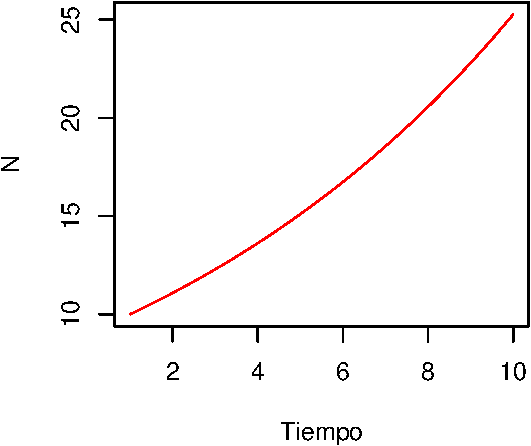
\includegraphics{Modelos-meta_files/figure-beamer/unnamed-chunk-1-1.pdf}
\end{frame}

\hypertarget{utilizando-r-para-hacer-integraciuxf3n-numuxe9rica}{%
\subsection{Utilizando R para hacer integración
numérica}\label{utilizando-r-para-hacer-integraciuxf3n-numuxe9rica}}

\begin{frame}[fragile]{Utilizando R para hacer integración numérica}
Iniciando valores

\begin{Shaded}
\begin{Highlighting}[]
\NormalTok{r }\OtherTok{\textless{}{-}} \FloatTok{0.1} \CommentTok{\#Parámetro}
\NormalTok{h }\OtherTok{\textless{}{-}} \FloatTok{0.5} \CommentTok{\#Longitud del paso}
\NormalTok{t }\OtherTok{\textless{}{-}} \DecValTok{10} \CommentTok{\#Número de unidades de tiempo}
\NormalTok{N }\OtherTok{\textless{}{-}} \FunctionTok{numeric}\NormalTok{(t}\SpecialCharTok{/}\NormalTok{h) }\CommentTok{\#Vector que contiene valores}
\NormalTok{N[}\DecValTok{1}\NormalTok{] }\OtherTok{\textless{}{-}} \DecValTok{10} \CommentTok{\#Tamaño inicial}
\end{Highlighting}
\end{Shaded}

Iteraciones de la integración

\begin{Shaded}
\begin{Highlighting}[]
\ControlFlowTok{for}\NormalTok{(i }\ControlFlowTok{in} \DecValTok{2}\SpecialCharTok{:}\FunctionTok{length}\NormalTok{(N))\{}
\NormalTok{      N[i] }\OtherTok{=}\NormalTok{ N[i}\DecValTok{{-}1}\NormalTok{] }\SpecialCharTok{+}\NormalTok{ r}\SpecialCharTok{*}\NormalTok{N[i}\DecValTok{{-}1}\NormalTok{]}\SpecialCharTok{*}\NormalTok{h}
\NormalTok{  \}}
\end{Highlighting}
\end{Shaded}
\end{frame}

\hypertarget{modelos-buxe1sicos-de-metapoblaciones}{%
\section{Modelos básicos de
metapoblaciones}\label{modelos-buxe1sicos-de-metapoblaciones}}

\hypertarget{el-concepto}{%
\subsection{El concepto}\label{el-concepto}}

\begin{frame}{El concepto}
\begin{center}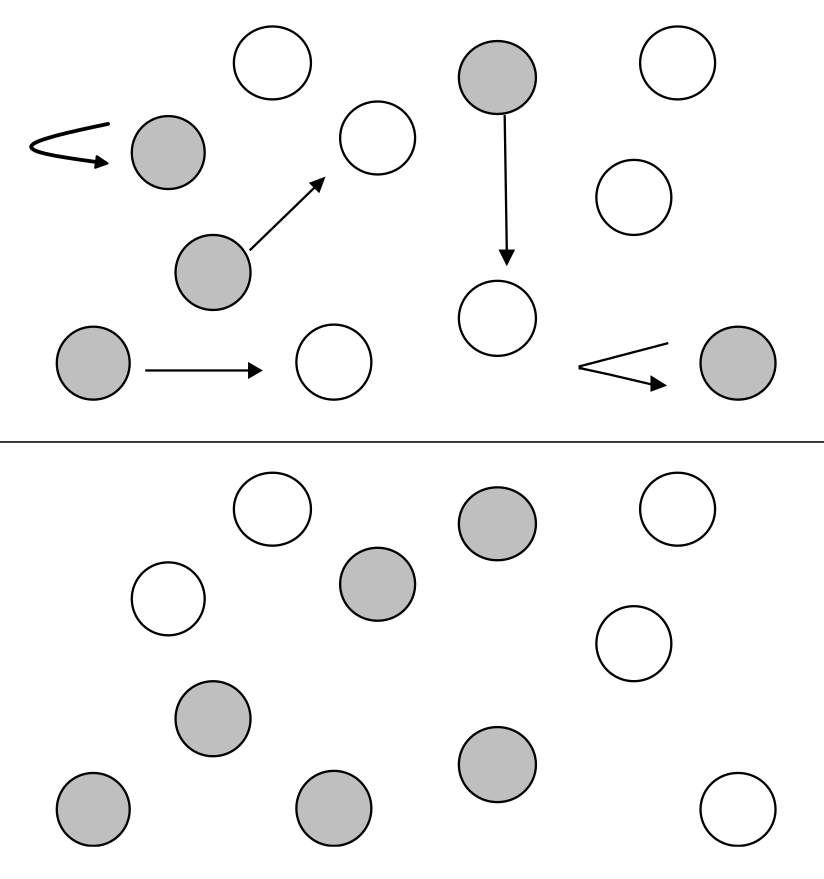
\includegraphics{Metapoblaciones/MEtap-May} \end{center}
\end{frame}

\hypertarget{el-concepto-1}{%
\subsection{El concepto}\label{el-concepto-1}}

\begin{frame}{El concepto}
\begin{itemize}
\item
  Representar proporción de parches de hábitat con presencia de la
  especie
\item
  Equilibrio entre colonizaciones y extinciones locales
\item
  Parches que emiten y parches que reciben individuos
\end{itemize}
\end{frame}

\hypertarget{poblaciones-fuente-y-sumidero}{%
\subsection{Poblaciones fuente y
sumidero}\label{poblaciones-fuente-y-sumidero}}

\begin{frame}{Poblaciones fuente y sumidero}
\begin{figure}

{\centering 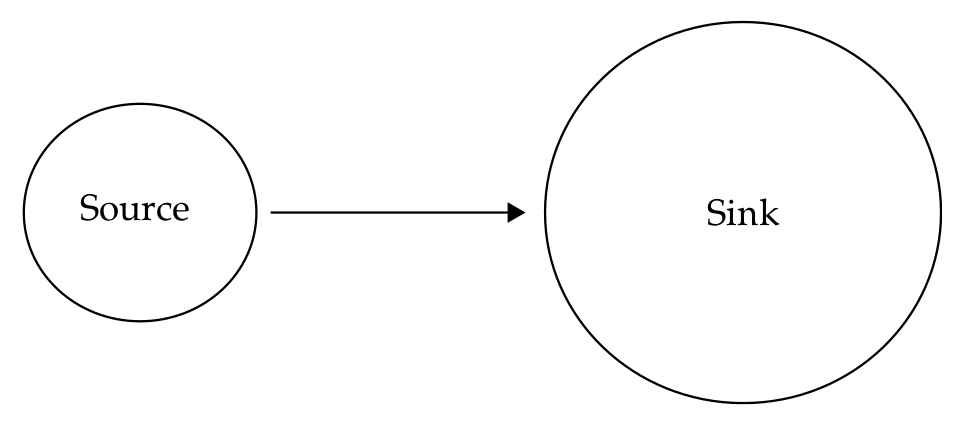
\includegraphics{Metapoblaciones/Fuente-sumidero} 

}

\caption{Poblaciones con r>0 son fuente. Poblaciones con r<0 son sumideros, las cuales persisten gracias a la inmigración.}\label{fig:unnamed-chunk-5}
\end{figure}
\end{frame}

\hypertarget{modelo-de-levins}{%
\subsection{Modelo de Levins}\label{modelo-de-levins}}

\begin{frame}{Modelo de Levins}
\begin{itemize}
\item
  Representa proporción de parches de hábitat ocupados por una especie
\item
  Parches ocupados dependen de parches ocupados:
\end{itemize}

\[\frac{dp}{dt} = cp(1-p)\]

\begin{itemize}
\item
  \(p\) es la proporción de parches ocupados
\item
  \(c\) es la tasa de colonización
\end{itemize}
\end{frame}

\hypertarget{racional}{%
\subsection{Racional}\label{racional}}

\begin{frame}{Racional}
\begin{itemize}
\item
  El máximo de parches ocupados es 1
\item
  La colonización disminuye si hay muchos ocupados

  \begin{itemize}
  \tightlist
  \item
    Baja probabilidad de encontrar parches desocupados
  \end{itemize}
\end{itemize}
\end{frame}

\hypertarget{integraciuxf3n}{%
\subsection{Integración}\label{integraciuxf3n}}

\begin{frame}[fragile]{Integración}
\begin{Shaded}
\begin{Highlighting}[]
\NormalTok{c }\OtherTok{\textless{}{-}} \FloatTok{0.5}\NormalTok{; h }\OtherTok{\textless{}{-}} \FloatTok{0.5}\NormalTok{; t }\OtherTok{\textless{}{-}} \DecValTok{20}
\NormalTok{p }\OtherTok{\textless{}{-}} \FunctionTok{numeric}\NormalTok{(t}\SpecialCharTok{/}\NormalTok{h); p[}\DecValTok{1}\NormalTok{] }\OtherTok{\textless{}{-}} \FloatTok{0.1}
\ControlFlowTok{for}\NormalTok{(i }\ControlFlowTok{in} \DecValTok{2}\SpecialCharTok{:}\FunctionTok{length}\NormalTok{(p))\{}
\NormalTok{  p[i] }\OtherTok{\textless{}{-}}\NormalTok{ p[i}\DecValTok{{-}1}\NormalTok{] }\SpecialCharTok{+}\NormalTok{ c}\SpecialCharTok{*}\NormalTok{p[i}\DecValTok{{-}1}\NormalTok{]}\SpecialCharTok{*}\NormalTok{(}\DecValTok{1}\SpecialCharTok{{-}}\NormalTok{p[i}\DecValTok{{-}1}\NormalTok{]) }\SpecialCharTok{*}\NormalTok{ h}
\NormalTok{\}}
\end{Highlighting}
\end{Shaded}
\end{frame}

\hypertarget{integraciuxf3n-1}{%
\subsection{Integración}\label{integraciuxf3n-1}}

\begin{frame}{Integración}
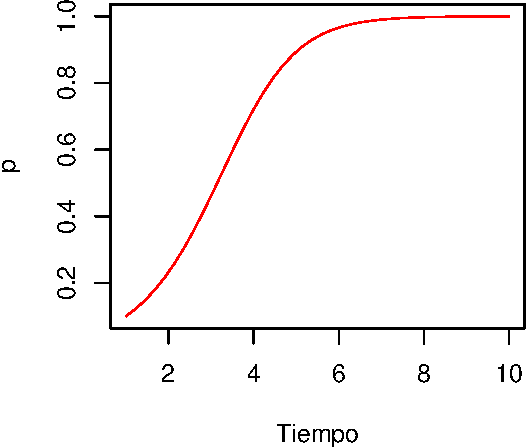
\includegraphics{Modelos-meta_files/figure-beamer/unnamed-chunk-7-1.pdf}
\end{frame}

\hypertarget{condiciones-de-estabilidad}{%
\subsection{Condiciones de
estabilidad}\label{condiciones-de-estabilidad}}

\begin{frame}{Condiciones de estabilidad}
\begin{itemize}
\tightlist
\item
  Sistema es estable cuando \(dp/dt = 0\)
\end{itemize}

\[cp(1-p) = 0\]

\begin{itemize}
\tightlist
\item
  Por lo tanto hay dos puntos en que la fracción de parches se mantiene
  constante:
\end{itemize}

\begin{enumerate}
\item
  \(p = 0\)
\item
  \(p = 1\)
\end{enumerate}
\end{frame}

\hypertarget{supuestos-del-modelo}{%
\subsection{Supuestos del modelo}\label{supuestos-del-modelo}}

\begin{frame}{Supuestos del modelo}
\begin{itemize}
\item
  Los individuos de mueven aleatoriamente entre parches
\item
  Sólo hay colonizaciones
\item
  No hay extinciones
\item
  Se pueden incluir extinciones en el sistema:
\end{itemize}

\[ \frac{dp}{dt} = cp(1-p) - ep\]

\begin{itemize}
\tightlist
\item
  \(e\) es la tasa de extinción
\end{itemize}
\end{frame}

\hypertarget{puntos-de-equilibrio}{%
\subsection{Puntos de equilibrio}\label{puntos-de-equilibrio}}

\begin{frame}{Puntos de equilibrio}
\begin{enumerate}
\item
  ¿Cuántos hay?
\item
  ¿Por qué?
\item
  ¿Cuál(es) es(son)?
\item
  Utilizando el código del modelo simple, integra el modelo con tasa de
  extinción
\item
  ¿Qué otros aspectos importantes debería incluir in modelo de
  metapoblaciones?
\end{enumerate}
\end{frame}

\hypertarget{lluvia-de-propuxe1gulos}{%
\section{Lluvia de propágulos}\label{lluvia-de-propuxe1gulos}}

\hypertarget{diferencias-con-levins}{%
\subsection{Diferencias con Levins}\label{diferencias-con-levins}}

\begin{frame}{Diferencias con Levins}
\begin{itemize}
\item
  En modelo de Levins la fracción de parches ocupados siempre proviene
  de otros parches ocupados
\item
  Existe posibilidad de inmigración de propagulos de otras fuentes
\item
  Lluvia de propagulos sugiere eventos aleatorios de inmigración:
\end{itemize}

\[\frac{dp}{dt} = c (1-p) - ep\]

\begin{itemize}
\item
  \(c\) es la probabilidad de inmigración de otras fuentes
\item
  ¿Punto(s) de equilibrio?
\end{itemize}
\end{frame}

\hypertarget{puntos-de-equilibrio-1}{%
\subsection{Punto(s) de equilibrio}\label{puntos-de-equilibrio-1}}

\begin{frame}{Punto(s) de equilibrio}
\[p^* = \frac{c}{c-e}\]

Si \(c = 0.1\) y \(e = 0.05\)

\[p^* = \frac{0.1}{0.1+0.05} = 0.666...\]

Aprximadamente el 67\% de los parches permanecerán ocupados
contstantemente
\end{frame}

\hypertarget{modelo-de-levins-con-lluvia-de-propuxe1gulos}{%
\subsection{Modelo de Levins con lluvia de
propágulos}\label{modelo-de-levins-con-lluvia-de-propuxe1gulos}}

\begin{frame}{Modelo de Levins con lluvia de propágulos}
Modelo

\[\frac{dp}{dt} = (c + c_e p)(1-p) - ep\]

\begin{itemize}
\item
  \(c\) es la probabilidad de importación de propágulos
\item
  \(c_e\) es la tasa de colonización
\item
  \(e\) es la tasa de extinción
\end{itemize}
\end{frame}

\hypertarget{modelo-de-levins-con-efecto-de-rescate}{%
\subsection{Modelo de Levins con efecto de
rescate}\label{modelo-de-levins-con-efecto-de-rescate}}

\begin{frame}{Modelo de Levins con efecto de rescate}
\begin{itemize}
\item
  Rescate: probabilidad de extinción disminuye cuando la fracción
  ocupada de parches es alta.
\item
  \(E\) es la extinción total y es afectada por los parches desocupados
  (\(1-p\)):
\end{itemize}

\[E = -ep(1-p)\]

E incluimos en el modelo de Levins con lluvia de propágulos:

\[\frac{dp}{dt} = (c + c_e p)(1-p) - ep(1-p)\]
\end{frame}

\hypertarget{destrucciuxf3n-de-huxe1bitat}{%
\section{Destrucción de hábitat}\label{destrucciuxf3n-de-huxe1bitat}}

\hypertarget{racional-1}{%
\subsection{Racional}\label{racional-1}}

\begin{frame}{Racional}
\begin{itemize}
\item
  La destrucción de hábitats es el problema definitorio del antropoceno
\item
  ¿Cómo podemos tomarlo en cuenta para las metapoblaciones?
\item
  La destrucción de hábitats debería de afectar la probabilidad de
  inmigración

  \begin{itemize}
  \tightlist
  \item
    Mas destrucción, menos atractivos son los hábitats, menos
    inmigración
  \end{itemize}
\item
  En Levins, la inmigración disminuye con fracción ocupada, por lo
  tanto\ldots{}
\end{itemize}
\end{frame}

\hypertarget{el-modelo}{%
\subsection{El modelo}\label{el-modelo}}

\begin{frame}{El modelo}
Modificación del modelo clásico (sin lluvia de propágulos ni rescate)

\[\frac{dp}{dt} = cp(1-D-p) - ep\]

\begin{itemize}
\item
  donde \(D\) es la fracción de hábitats destruidos
\item
  Punto(s) de equilibrio:
\end{itemize}

\[p^* = 1 - \frac{e}{c} - D\]
\end{frame}

\end{document}
